\documentclass[11pt]{article}

\usepackage[margin=1in]{geometry}
\usepackage[T1]{fontenc}
\usepackage{graphicx}
\usepackage{booktabs}
\usepackage{amsmath}
\usepackage{amssymb}
\usepackage{xcolor}
\usepackage{float}
\usepackage{enumitem}
\usepackage{hyperref}
\usepackage{listings}

\graphicspath{{../assets/screenshots/}}
\hypersetup{colorlinks=true,linkcolor=blue!45!black,urlcolor=blue!45!black}
\setlength{\parskip}{0.65em}
\setlength{\parindent}{0pt}
\lstset{
  basicstyle=\ttfamily\small,
  breaklines=true,
  frame=single,
  columns=fullflexible,
  showstringspaces=false
}

\title{\textbf{PlanForge}\\A Constraint Satisfaction Framework for Apartment Floor-Plan Generation}
\author{Designed by Mohammad Saleh Mahdinejad\\Artificial Intelligence Fundamentals and Applications}
\date{\today}

\begin{document}
\maketitle

\begin{abstract}
PlanForge is an educational project that turns apartment floor-plan generation into a concrete
constraint satisfaction problem. Students receive a visual framework, a set of JSON problem
instances, a public self-check, and a small set of starter files. Their task is to implement the
search intelligence: recursive backtracking, consistency checks, variable and value ordering,
optional inference, and soft optimization. The project is designed to make CSP concepts visible:
each room placement becomes a domain value, each architectural rule becomes a constraint, and
the visual solver can replay the actual search path as a tree.
\end{abstract}

\tableofcontents
\newpage

\section{Project Motivation}

Classic CSP assignments often use abstract examples such as map coloring or n-queens. Those
examples are useful, but they can feel disconnected from the way constraints appear in real
design problems. PlanForge uses apartment planning as the domain: rooms must fit inside a
fixed shell, must not overlap, must satisfy adjacency and boundary requirements, and should
also produce a layout that looks reasonable.

The project has two goals. First, it gives students a strict CSP core where correctness can be
graded through hard constraints. Second, it gives advanced students room to improve search
quality through inference and soft scoring. This creates a clean separation between required
correctness and optional optimization.

\section{High-Level Workflow}

The framework separates problem definition, domain generation, student search, validation,
and visualization. This separation keeps the assignment fair: students implement the algorithmic
core, while the framework provides consistent loading, checking, rendering, and reporting.

\begin{figure}[H]
  \centering
  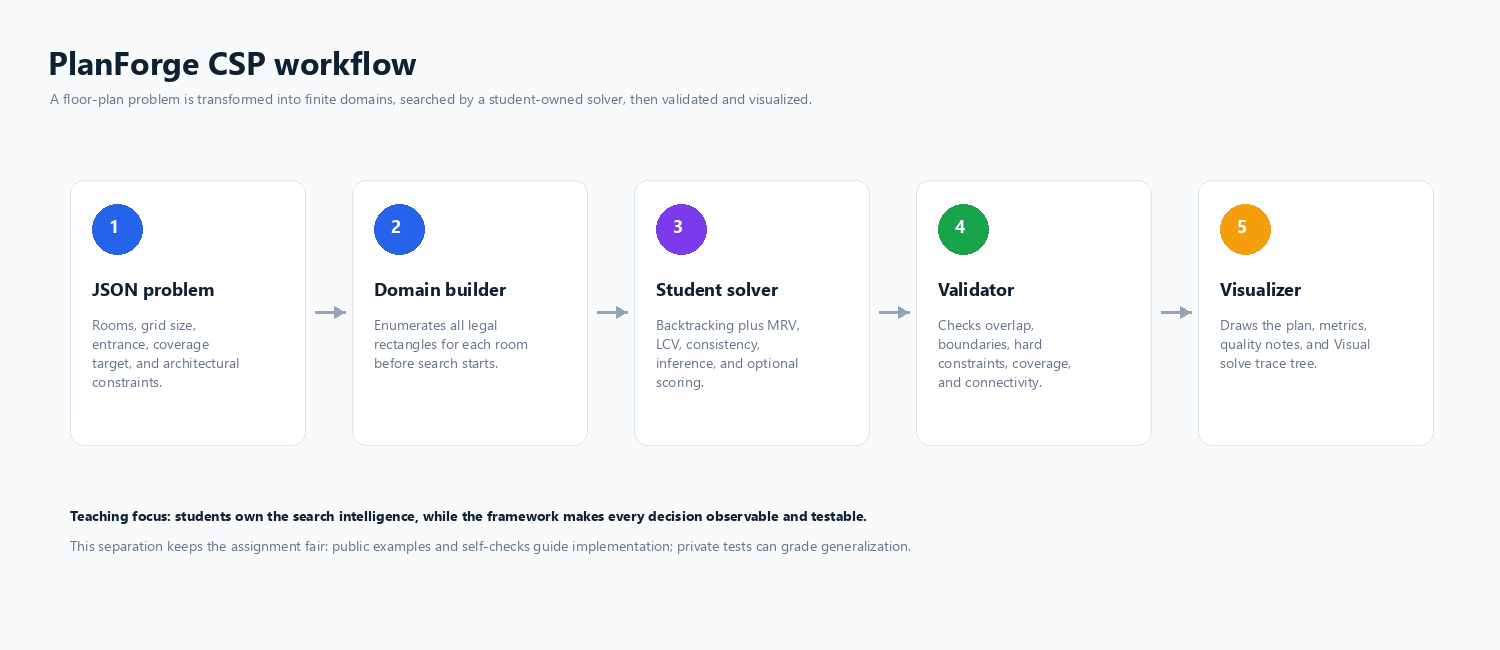
\includegraphics[width=\textwidth]{planforge-csp-workflow.png}
  \caption{PlanForge transforms a declarative floor-plan case into domains, runs the student solver, validates the result, and visualizes the outcome.}
\end{figure}

\section{CSP Formulation}

PlanForge models each apartment case as a finite-domain CSP:

\[
  \text{CSP} = (X, D, C)
\]

where:

\begin{itemize}[leftmargin=*]
  \item $X$ is the set of variables, one variable per room.
  \item $D_i$ is the finite domain of legal rectangles for room $i$.
  \item $C$ is the set of hard constraints that define validity.
\end{itemize}

Each domain value is a rectangle:

\[
  r = (x, y, w, h)
\]

where $x$ and $y$ are grid coordinates and $w$ and $h$ are integer dimensions. The domain
builder enumerates every rectangle that fits the room's area, width, height, aspect-ratio, and
boundary requirements.

\subsection{Variables}

The variables are room names such as \texttt{Hall}, \texttt{Bathroom}, \texttt{Living},
\texttt{Kitchen}, \texttt{Bedroom1}, \texttt{Storage}, or \texttt{Balcony}. A complete assignment
maps every room name to exactly one rectangle.

\subsection{Domains}

A room domain is not the entire grid. It is filtered before search begins. The framework removes
rectangles that violate room-level requirements such as:

\begin{itemize}[leftmargin=*]
  \item minimum and maximum area,
  \item minimum and maximum width,
  \item minimum and maximum height,
  \item maximum aspect ratio,
  \item exterior access when required.
\end{itemize}

This precomputation makes the search problem finite, explicit, and inspectable.

\subsection{Hard Constraints}

The validator and student consistency function work with constraints such as:

\begin{table}[H]
\centering
\begin{tabular}{ll}
\toprule
Constraint & Meaning \\
\midrule
\texttt{adjacent(a,b)} & Rooms must share a wall segment. \\
\texttt{not\_adjacent(a,b)} & Rooms must not share a wall segment. \\
\texttt{near\_entrance(room)} & Room must be close to the entrance point. \\
\texttt{far\_from\_entrance(room)} & Room must be sufficiently far from the entrance point. \\
\texttt{touches\_boundary(room)} & Room must touch the exterior boundary. \\
\texttt{touches\_wall(room, wall)} & Room must touch a specific shell wall. \\
\texttt{larger\_than(a,b)} & Room \texttt{a} must have greater area than room \texttt{b}. \\
\bottomrule
\end{tabular}
\caption{Representative PlanForge hard constraints.}
\end{table}

In addition to explicit JSON constraints, every valid solution must satisfy global requirements:
rectangles must stay inside the shell, rooms must not overlap, coverage must exceed the required
threshold, and the final room adjacency graph must be connected when connectivity is required.

\section{JSON Problem Format}

Each example is stored under \texttt{planforge/examples/}. The JSON schema is intentionally
simple enough for students to read while still expressing meaningful design cases.

\begin{lstlisting}[caption={Simplified example of a PlanForge problem.}]
{
  "width": 10,
  "height": 8,
  "entrance": [0, 7],
  "minCoverageRatio": 0.72,
  "requireConnected": true,
  "rooms": [
    {
      "name": "Living",
      "minArea": 16,
      "maxArea": 20,
      "minW": 4,
      "maxW": 5,
      "minH": 4,
      "maxH": 4,
      "needsExterior": true
    }
  ],
  "constraints": [
    {"type": "adjacent", "a": "Living", "b": "Kitchen"},
    {"type": "near_entrance", "room": "Hall", "max_distance": 3}
  ]
}
\end{lstlisting}

The visible examples cover easy, medium, hard, unsatisfiable, and bonus challenge scenarios.
The unsatisfiable case is important because it prevents students from assuming that every search
must return a layout.

\section{Framework Architecture}

The public repository is organized around a small framework and a student-owned work area.

\begin{table}[H]
\centering
\begin{tabular}{ll}
\toprule
Path & Responsibility \\
\midrule
\texttt{planforge/core/models.py} & Dataclasses for rectangles, room specs, constraints, and CSP problems. \\
\texttt{planforge/core/domain\_builder.py} & Enumerates finite rectangle domains for each room. \\
\texttt{planforge/core/geometry.py} & Geometry utilities: overlap, adjacency, distance, connectivity. \\
\texttt{planforge/core/constraints.py} & Parses and evaluates hard constraints. \\
\texttt{planforge/core/loader.py} & Loads JSON cases into \texttt{CSPProblem} objects. \\
\texttt{planforge/core/validator.py} & Validates complete assignments. \\
\texttt{planforge/core/quality.py} & Computes architectural soft quality scores. \\
\texttt{planforge/core/engine.py} & Runs the student solver and records instrumentation. \\
\texttt{planforge/core/visualizer.py} & Tkinter studio, layout canvas, metrics, JSON viewer, Visual solve. \\
\texttt{student/} & Student TODO files. \\
\bottomrule
\end{tabular}
\caption{Main repository modules and their roles.}
\end{table}

\section{Student Implementation Surface}

Students are expected to edit only the \texttt{student/} package. The starter files expose the
algorithmic hooks without hiding the important CSP responsibilities.

\subsection{Required Files}

\begin{itemize}[leftmargin=*]
  \item \texttt{student/solver.py}: implement \texttt{solve}, \texttt{backtrack}, and \texttt{is\_complete}.
  \item \texttt{student/consistency.py}: implement partial-assignment consistency checking.
  \item \texttt{student/heuristics.py}: implement MRV and LCV.
\end{itemize}

\subsection{Optional Files}

\begin{itemize}[leftmargin=*]
  \item \texttt{student/inference.py}: implement forward checking and AC-3.
  \item \texttt{student/scoring.py}: implement a soft layout score used to choose the best valid plan.
\end{itemize}

The framework grades only the student-owned interface. This makes it possible to test submissions
inside a clean scaffold and prevents students from gaining credit by modifying the visualizer,
examples, or public grader.

\section{Backtracking and Instrumentation}

The student solver receives a \texttt{SolverContext}. This object records search statistics and
provides hooks that make the algorithm visible.

\begin{lstlisting}[language=Python,caption={Typical instrumentation calls inside recursive backtracking.}]
ctx.on_node()
variable = select_unassigned_variable(problem, assignment, domains)
ctx.on_select_variable(variable, assignment)

for value in order_domain_values(problem, variable, assignment, domains):
    ctx.on_assignment_tried()
    ctx.on_consistency_check()
    if is_consistent(problem, assignment, variable, value):
        assignment[variable] = value
        ctx.on_assign(variable, value, assignment)
        ...
        del assignment[variable]
        ctx.on_unassign(variable, assignment)

ctx.on_backtrack()
\end{lstlisting}

These calls do not solve the CSP for the student. They only expose the student's own decisions
to the framework. This is useful for grading, debugging, and the Visual solve mode.

\section{Visual Solve Mode}

PlanForge includes a graphical mode that replays the search trace. When tracing is enabled,
the UI displays the current apartment assignment and a DFS tree representing the explored
search path. Current branches, solutions, pruned domains, and backtracked nodes use different
visual encodings.

\begin{figure}[H]
  \centering
  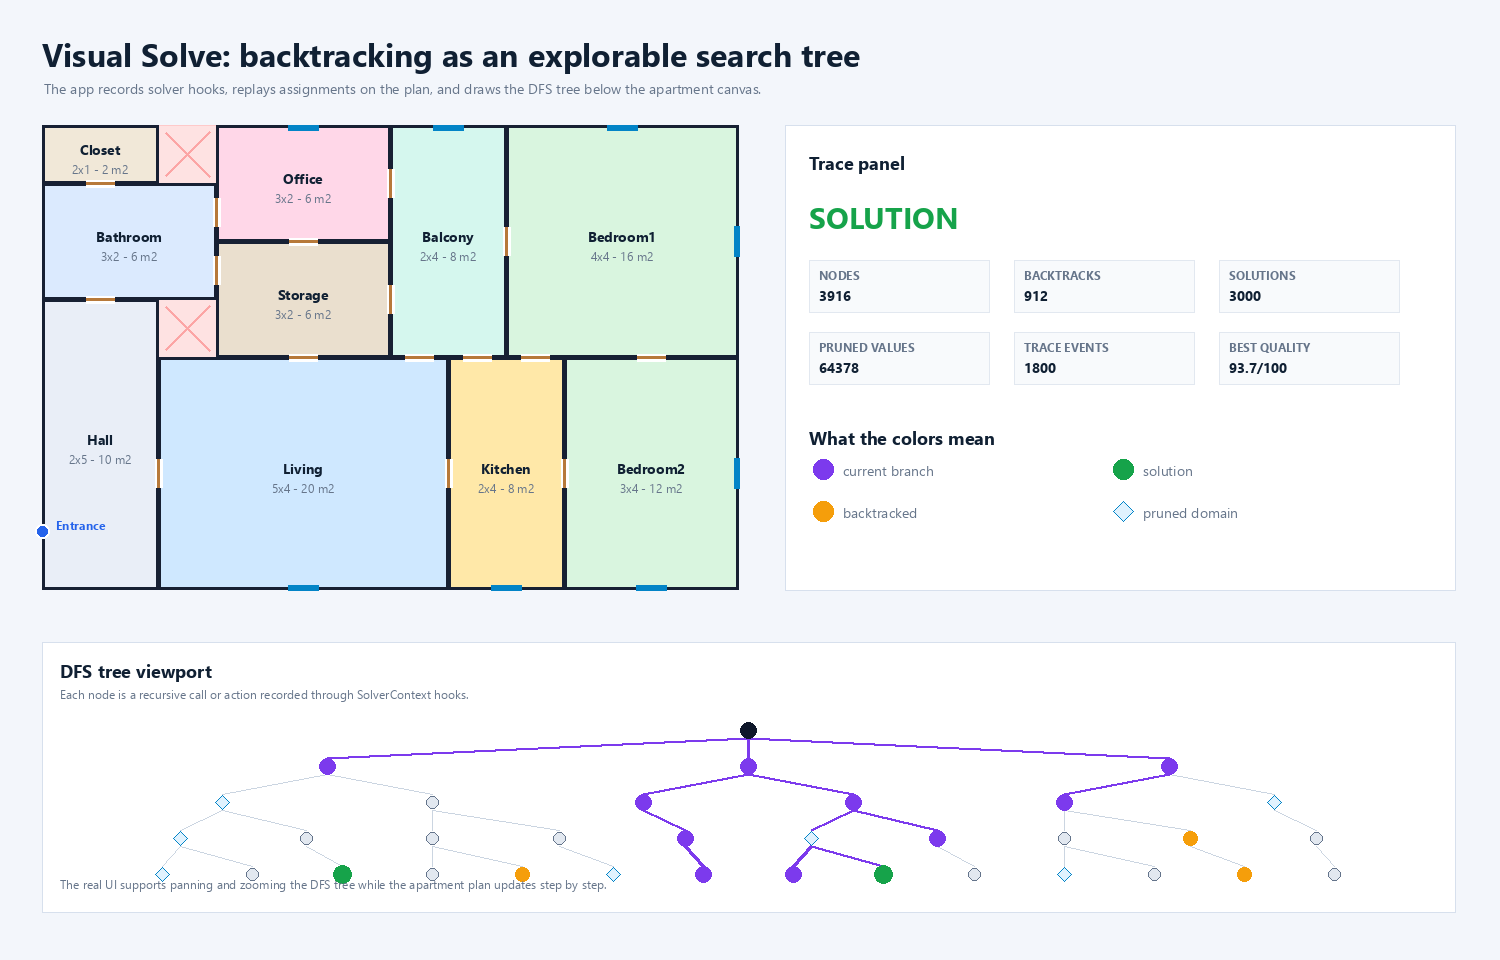
\includegraphics[width=\textwidth]{planforge-visual-solve-tree.png}
  \caption{Visual solve mode shows the generated apartment and a DFS search tree driven by \texttt{SolverContext} trace hooks.}
\end{figure}

This mode is valuable pedagogically because it turns backtracking from a hidden recursive process
into an observable sequence. Students can see how MRV changes variable selection, how LCV changes
branch order, how inference prunes candidate values, and why a branch fails.

\section{Layout Visualization}

The main studio view displays the selected case, solver status, metrics, and the generated
floor plan. Rooms are rendered as colored rectangles. Doors are drawn between adjacent rooms,
windows are shown on exterior-facing rooms, and unused cells are highlighted.

\begin{figure}[H]
  \centering
  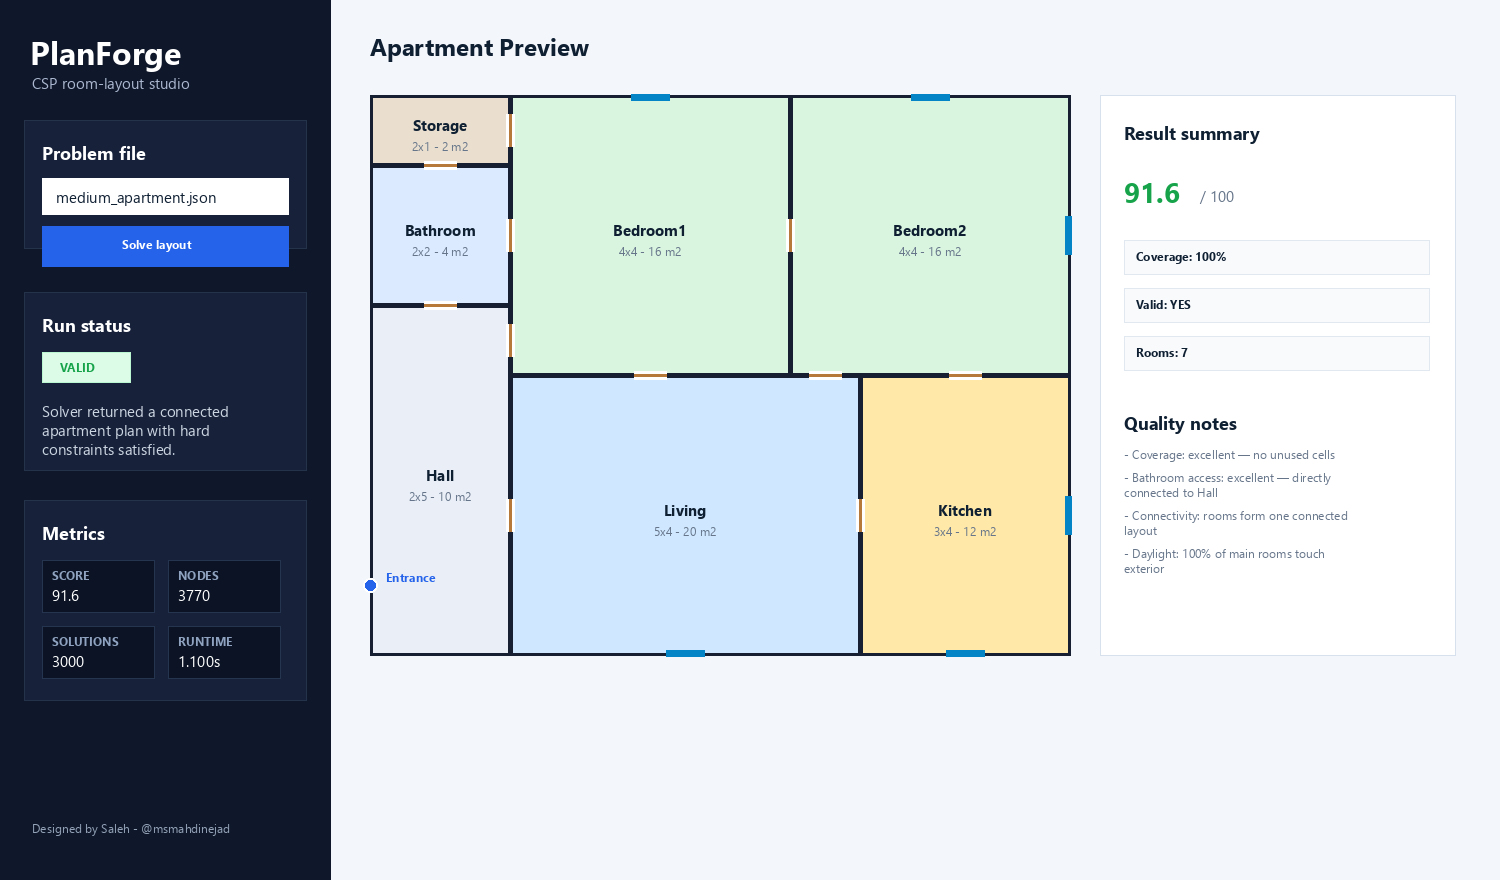
\includegraphics[width=\textwidth]{planforge-studio-medium.png}
  \caption{The desktop studio view for a solved medium apartment case.}
\end{figure}

The visualization intentionally includes both correctness and quality signals. A layout can be
valid while still having a weak quality score, which helps students understand the difference
between hard constraints and soft objectives.

\section{Quality Scoring}

Validity and quality are separate. A valid solution satisfies all hard constraints. A high-quality
solution also reflects architectural preferences. The framework-owned quality score considers:

\begin{itemize}[leftmargin=*]
  \item coverage and unused area,
  \item public circulation from entrance to hall and living room,
  \item bathroom accessibility,
  \item connected room graph,
  \item public/private zoning,
  \item daylight and exterior access,
  \item room shape compactness,
  \item preferred adjacencies such as living-kitchen and kitchen-balcony.
\end{itemize}

Students can implement \texttt{score\_assignment} to guide selection among multiple valid
assignments. This creates a natural advanced path: after finding any solution, students can
search for better solutions.

\section{Public Self-Check}

The public grader is included as a visible feedback tool. It checks importability, basic heuristic
behavior, public example solutions, unsatisfiable detection, instrumentation, and optional
performance behavior. It is explicitly not the final grader.

\begin{figure}[H]
  \centering
  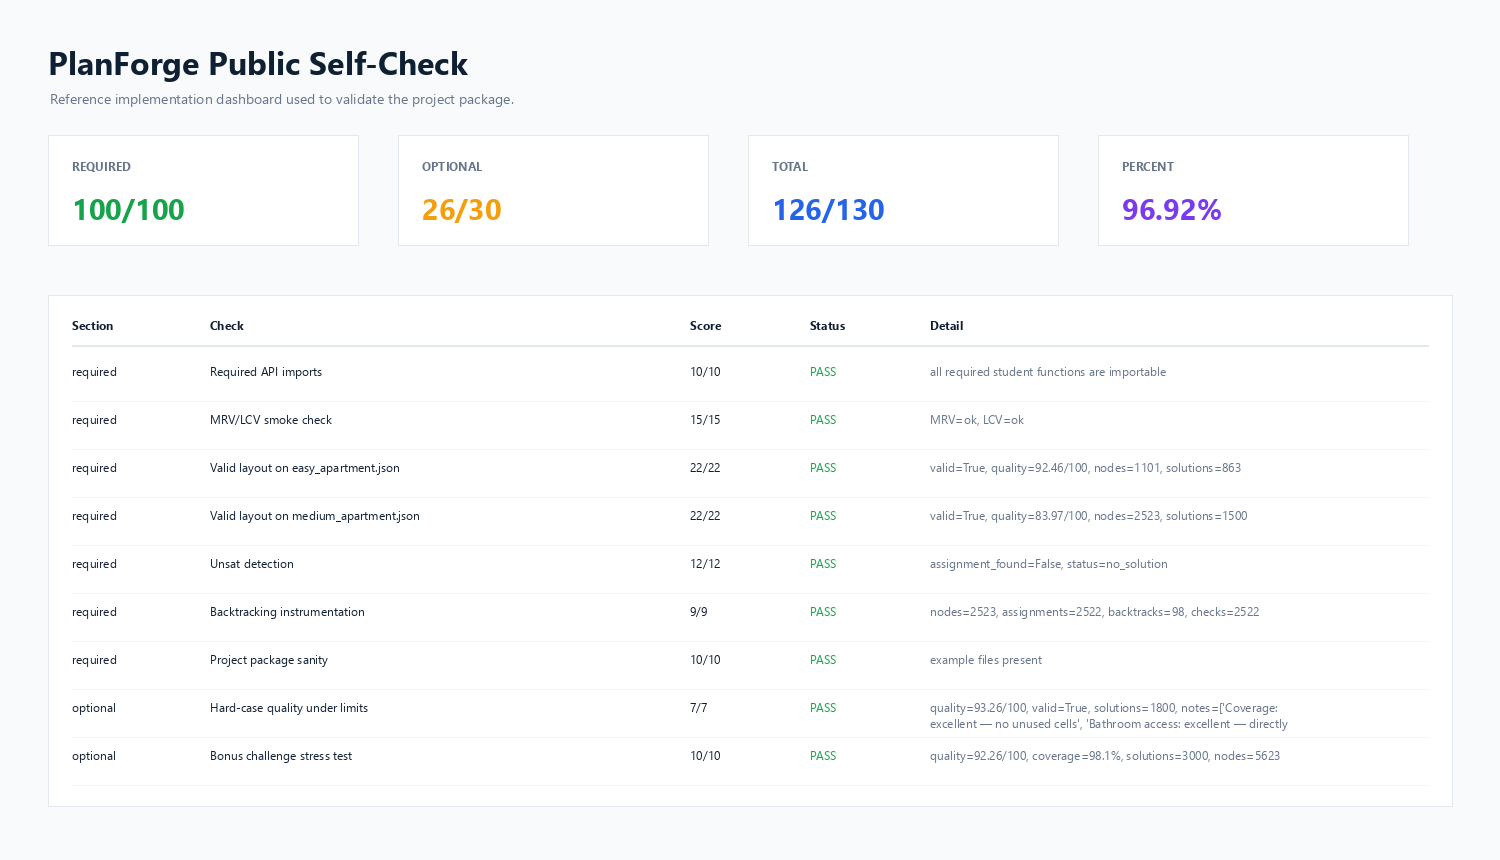
\includegraphics[width=\textwidth]{planforge-public-grade.png}
  \caption{Public self-check dashboard generated from the reference implementation.}
\end{figure}

The final grading policy should use private cases and a private grader. This protects the
assignment from overfitting to visible examples while still giving students enough public feedback
to debug their implementations.

\section{Required and Optional Grading}

The assignment is structured as 100 required points and 30 optional points.

\begin{table}[H]
\centering
\begin{tabular}{lll}
\toprule
Section & Focus & Examples \\
\midrule
Required & Correct CSP search & Backtracking, consistency, MRV, LCV, valid public layouts. \\
Required & Robustness & Unsatisfiable-case detection and instrumentation. \\
Optional & Inference & Forward checking, AC-3, stronger pruning. \\
Optional & Optimization & Multi-solution search and soft layout scoring. \\
\bottomrule
\end{tabular}
\caption{Grading categories in PlanForge.}
\end{table}

\section{Recommended Student Strategy}

A practical implementation path is:

\begin{enumerate}[leftmargin=*]
  \item Implement \texttt{is\_complete}.
  \item Implement a simple recursive backtracking solver using raw domain order.
  \item Implement \texttt{is\_consistent} for boundaries, area, overlap, and checkable constraints.
  \item Add \texttt{ctx} instrumentation so the public grader and visualizer can observe the search.
  \item Add MRV and LCV.
  \item Add forward checking.
  \item Add AC-3 if time allows.
  \item Implement \texttt{score\_assignment} and keep searching for better valid layouts.
\end{enumerate}

This sequence gives students early visible progress while leaving enough depth for advanced work.

\section{Public Repository Policy}

The public repository should contain the starter package, visualizer, public examples, public
self-check, screenshots, and documentation. It should not contain private grader logic, hidden
tests, private grade reports, batch grading outputs, or reference solution source code.

This is why the repository is designed as a clean public release rather than a full instructor
archive. The public materials teach and guide; the private materials grade and audit.

\section{Conclusion}

PlanForge connects CSP theory to a concrete design problem. It preserves the core ideas of AI
search while giving students visual feedback and a meaningful optimization target. The result is
an assignment where algorithmic choices are visible: variable ordering changes the tree, inference
shrinks the search space, and soft scoring improves the final layout.

\end{document}
